\section{Optimal polynomial--wise constraint ratio}
\subsection{Inf--sup value estimator}

Without loss generality, the incompressible elasticity problem is considered herein to illustrate the proposed methodology.
The approximations of Eq.\eqref{} should satisfy the inf-sup condition, or as known Ladyzhenskaya–Babuška–Brezzi condition \cite{bathe1996}, to ensure the formulation's accuracy:
\begin{equation}\label{infsup}
    \inf_{q_h \in Q_h} \sup_{\boldsymbol v_h \in V_h} \frac{\vert b(q_h,\boldsymbol v_h) \vert}{\Vert q_h \Vert_Q \Vert \boldsymbol v_h \Vert_V} \ge \beta > 0
\end{equation}
in which $\beta$, namely inf-sup value, is a constant independent of characterized element size $h$.

\begin{thm}\label{thm1}
Suppose $\mathcal P_h:V_h \rightarrow Q_h$ is the orthogonal projection operator of $\mathcal P$ defined by:
\begin{equation}\label{Ph}
    b(q_h,\boldsymbol v_h) = (q_h, \mathcal P \boldsymbol v_h) = (q_h, \mathcal P_h \boldsymbol v_h), \quad \forall q_h \in Q_h
\end{equation}
where $\mathcal P:V\rightarrow Q$ is the divergence operator, $\mathcal P = \nabla \cdot$. And the inf-sup value can be estimated by:
\begin{equation}\label{r1}
    \beta \le \inf_{V'_h \subset V_h \setminus \ker \mathcal P_h} \sup_{v_h \in V'_h} \frac{\Vert \mathcal P_h \boldsymbol v_h \Vert_Q}{\Vert \boldsymbol v_h \Vert_V}
\end{equation}
    where $\ker \mathcal P_h \subset V$ is the kernel of $\mathcal P_h$ defined by $\ker \mathcal P_h := \{ \boldsymbol v \in V \;\vert\; \mathcal P_h \boldsymbol v = 0 \}$.
\end{thm}
\begin{pf}
As the definition of  $\mathcal P_h$, we have $\mathrm{Im}\mathcal P_h \in Q_h$. And the Eq. \eqref{infsup} can be rewritten as:
\begin{equation} \label{r11}
\begin{split}
    \beta &\le \inf_{q_h \in Q_h} \sup_{\boldsymbol v_h \in V_h} \frac{\vert b(q_h,\boldsymbol v_h) \vert}{\Vert q_h \Vert_Q \Vert \boldsymbol v_h \Vert_V} 
    \le \inf_{q_h \in \mathrm{Im}\mathcal P_h} \sup_{\boldsymbol v_h \in V_h} \frac{\vert (q_h,\mathcal P_h \boldsymbol v_h) \vert}{\Vert q_h \Vert_Q \Vert \boldsymbol v_h \Vert_V} \\
\end{split}
\end{equation}

For a given $q_h\in \mathrm{Im}\mathcal P_h$, suppose a space $V'_h \subset V_h\setminus \ker P_h$ defined by:
\begin{equation}
    V'_h = \{ \boldsymbol v_h \in V_h \; \vert \; \mathcal P_h \boldsymbol v_h = q_h \}
\end{equation}
Since $\mathrm{Im}\mathcal P_h \in Q_h$, in accordance with Cauchy-Schwarz inequality, we have:
\begin{equation}
    \vert (q_h,\mathcal P_h \boldsymbol v_h) \vert \le \Vert q_h \Vert_Q \Vert \mathcal P_h \boldsymbol v_h \Vert_Q
\end{equation}
where this equality is holding if and only if $q_h=\mathcal P_h \boldsymbol v_h$, i.e.,
\begin{equation}
    \vert (q_h,\mathcal P_h \boldsymbol v_h) \vert = \Vert q_h \Vert_Q \Vert \mathcal P_h \boldsymbol v_h \Vert_Q, \quad \forall \boldsymbol v_h \in V'_h
\end{equation}
And the following relationship can be evidenced:
    \begin{equation}\label{r12}
    \sup_{\boldsymbol v_h\in V_h} \frac{\vert (q_h,\mathcal P_h \boldsymbol v_h) \vert}{\Vert q_h \Vert_Q \Vert \boldsymbol v_h \Vert_V} =
    \sup_{\boldsymbol v_h\in V'_h} \frac{\Vert \mathcal P_h \boldsymbol v_h \Vert_Q}{\Vert \boldsymbol v_h \Vert_V} 
\end{equation}

Consequently, with a combination of Eqs. \eqref{r11} and \eqref{r12}, Eq. \eqref{r1} can be obtain.
\end{pf}

\begin{rmk}
Theorem \ref{thm1} is consistance with the traditional numerical inf-sup test \cite{malkus1981}, while, according to minimum-maximum principle \cite{babuska1991a}, the Eq. \eqref{r1} evaluates the general non-zero eigenvalue of metrics $\boldsymbol K^v$ and $\boldsymbol K^d$.
\end{rmk}

In order to further figure out the optimal constraint counting ,
\begin{thm}
    Suppose that $P_{n_u}$ is a polynomial space with $n_u$ dimensions, and $V_{n_u}$ is the polynomial displacement space, $V_{n_u} = P_{n_u}^2$. The optimal dofs of pressure $n_p$ is equal to $n_c = \dim(V_{n_c}\setminus \ker \mathcal P)$.
\end{thm}
\begin{pf}
    As the dimensions of $V_h$ and $V_{n_u}$ is identical, $\dim V_{n_u}=\dim V_h = n_d\times n_u$. There exists a unique $\boldsymbol v \in V_{n_u}$ satisfing $\boldsymbol v_h = \mathcal I_h \boldsymbol v$. And the right side of Eq. \eqref{r1} becomes:
\begin{equation}\label{r21}
\inf_{V'_h \subset V_h\setminus \ker \mathcal P_h}\sup_{\boldsymbol v_h \in V_h'} \frac{\Vert \mathcal P_h \boldsymbol v_h \Vert_Q}{\Vert \boldsymbol v_h \Vert_V} = 
\inf_{V'\subset V_{n_u}\setminus \ker \mathcal P_h \mathcal I_h}\sup_{\boldsymbol v \in V'} \frac{\Vert \mathcal P_h \mathcal I_h \boldsymbol v \Vert_Q}{\Vert \mathcal I_h \boldsymbol v \Vert_V}
\end{equation}

In accordance with triangular inequality, Cauchy-Schwarz inequality and the relationship of Eqs. \eqref{Ph}, we have:
\begin{equation}\label{interpolation1}
\begin{split}
    \Vert \mathcal P_h \mathcal I_h \boldsymbol v \Vert_Q &= 
    \sup_{q_h \in Q_h} \frac{\vert (q_h, \mathcal P_h \mathcal I_h \boldsymbol v) \vert}{\Vert q_h \Vert_Q}
    =\sup_{q_h \in Q_h} \frac{\vert (q_h, \mathcal P \mathcal I_h \boldsymbol v) \vert}{\Vert q_h \Vert_Q} \\
    &\le \sup_{q_h \in Q_h} \frac{\vert (q_h, \mathcal P \boldsymbol v)\vert + \vert (q_h, \mathcal P \boldsymbol v - \mathcal P \mathcal I_h \boldsymbol v) \vert}{\Vert q_h \Vert_Q} \\
    &= \Vert \mathcal P_h \boldsymbol v \Vert_Q
    + \Vert \mathcal P(\mathcal I - \mathcal I_h) \boldsymbol v \Vert_Q \\
    &\le C \Vert \mathcal P \boldsymbol v \Vert_Q
    + \Vert \mathcal P(\mathcal I - \mathcal I_h) \boldsymbol v \Vert_Q 
\end{split}
\end{equation}
Obviously, the second and third terms on the right side of Eq. \eqref{interpolation1} are the interpolation error and the orthogonal projection error for approximations in $V_h$, and can be evaluated by \cite{yosida1995}:
\begin{equation}
\label{interpolation2}
    \Vert \mathcal P(\mathcal I - \mathcal I_h) \boldsymbol v \Vert_Q \le Ch^k \vert \boldsymbol v \vert_{H^k} 
\end{equation}
    It can be obtained that $\Vert \mathcal I_h \boldsymbol v\Vert_V \ge C\Vert \boldsymbol v \Vert_V$ from close graph theorem \cite{quarteroni1994}. And considering it with Eqs. \eqref{interpolation1}-\eqref{interpolation2}, the right side of Eq. \eqref{r21} can be represented as:
\begin{equation}\label{r23}
\begin{split}
    \inf_{V'\subset V_{n_u}\setminus \ker \mathcal P_h \mathcal I_h} \sup_{\boldsymbol v \in V'} \frac{\Vert \mathcal P_h\mathcal I_h\boldsymbol v\Vert_Q}{\Vert \mathcal I_h \boldsymbol v\Vert_V} 
    &\le \inf_{V'\subset V_{n_u}\setminus \ker \mathcal P_h \mathcal I_h} \sup_{\boldsymbol v \in V'} \frac{\Vert \mathcal P_h \boldsymbol v\Vert_Q}{\Vert \boldsymbol v\Vert_V} + Ch^k \\
    &\le C \inf_{V'\subset V_{n_u}\setminus \ker \mathcal P_h \mathcal I_h} \sup_{\boldsymbol v \in V'} \frac{\Vert \mathcal P\boldsymbol v\Vert_Q}{\Vert \boldsymbol v\Vert_V} + Ch^k \\
\end{split}
\end{equation}
Substituting Eqs. \eqref{r21},\eqref{r23} into \eqref{r1} can get the following relationship:
\begin{equation}\label{r3}
\begin{split}
    \beta &\le \beta_1 + Ch^k \\
    &\le C \beta_2 + Ch^k
\end{split}
\end{equation}
where
\begin{align}
    \beta_1 &= \inf_{V'\subset V_{n_u}\setminus\ker \mathcal P_h \mathcal I_h}\sup_{\boldsymbol v \in V'}\frac{\Vert \mathcal P_h \boldsymbol v\Vert_Q}{\Vert \mathcal I_h \boldsymbol v\Vert_V} \\
    \beta_2 &= \inf_{V'\subset V_{n_u}\setminus\ker \mathcal P_h \mathcal I_h}\sup_{\boldsymbol v \in V'}\frac{\Vert \mathcal P \boldsymbol v\Vert_Q}{\Vert\boldsymbol v\Vert_V} \\
\end{align}

    As illstrated in Figure \ref{}, due to the approximations' partition of unity property, the sub-spaces $\ker \mathcal P$, $\ker \mathcal P_h$ and $\ker \mathcal P_h \mathcal I_h$ is arranged gathering at one side on $V_{n_u}$, where $n_p = \dim(V_{n_u}\setminus \ker \mathcal P_h \mathcal I_h) \le n_d \times n_u$. 
    Let $n_c = \dim(V_{n_u}\setminus \ker \mathcal P)$, $n_h = \dim(V_{n_u}\setminus \ker \mathcal P I_h)$, 
    it is obvious that $\ker \mathcal P \subseteq \ker \mathcal P \mathcal I_h$, $n_h \le n_c$.
    The different choices of $n_p$ will appear the following three cases:

\begin{figure}[!ht]
\centering
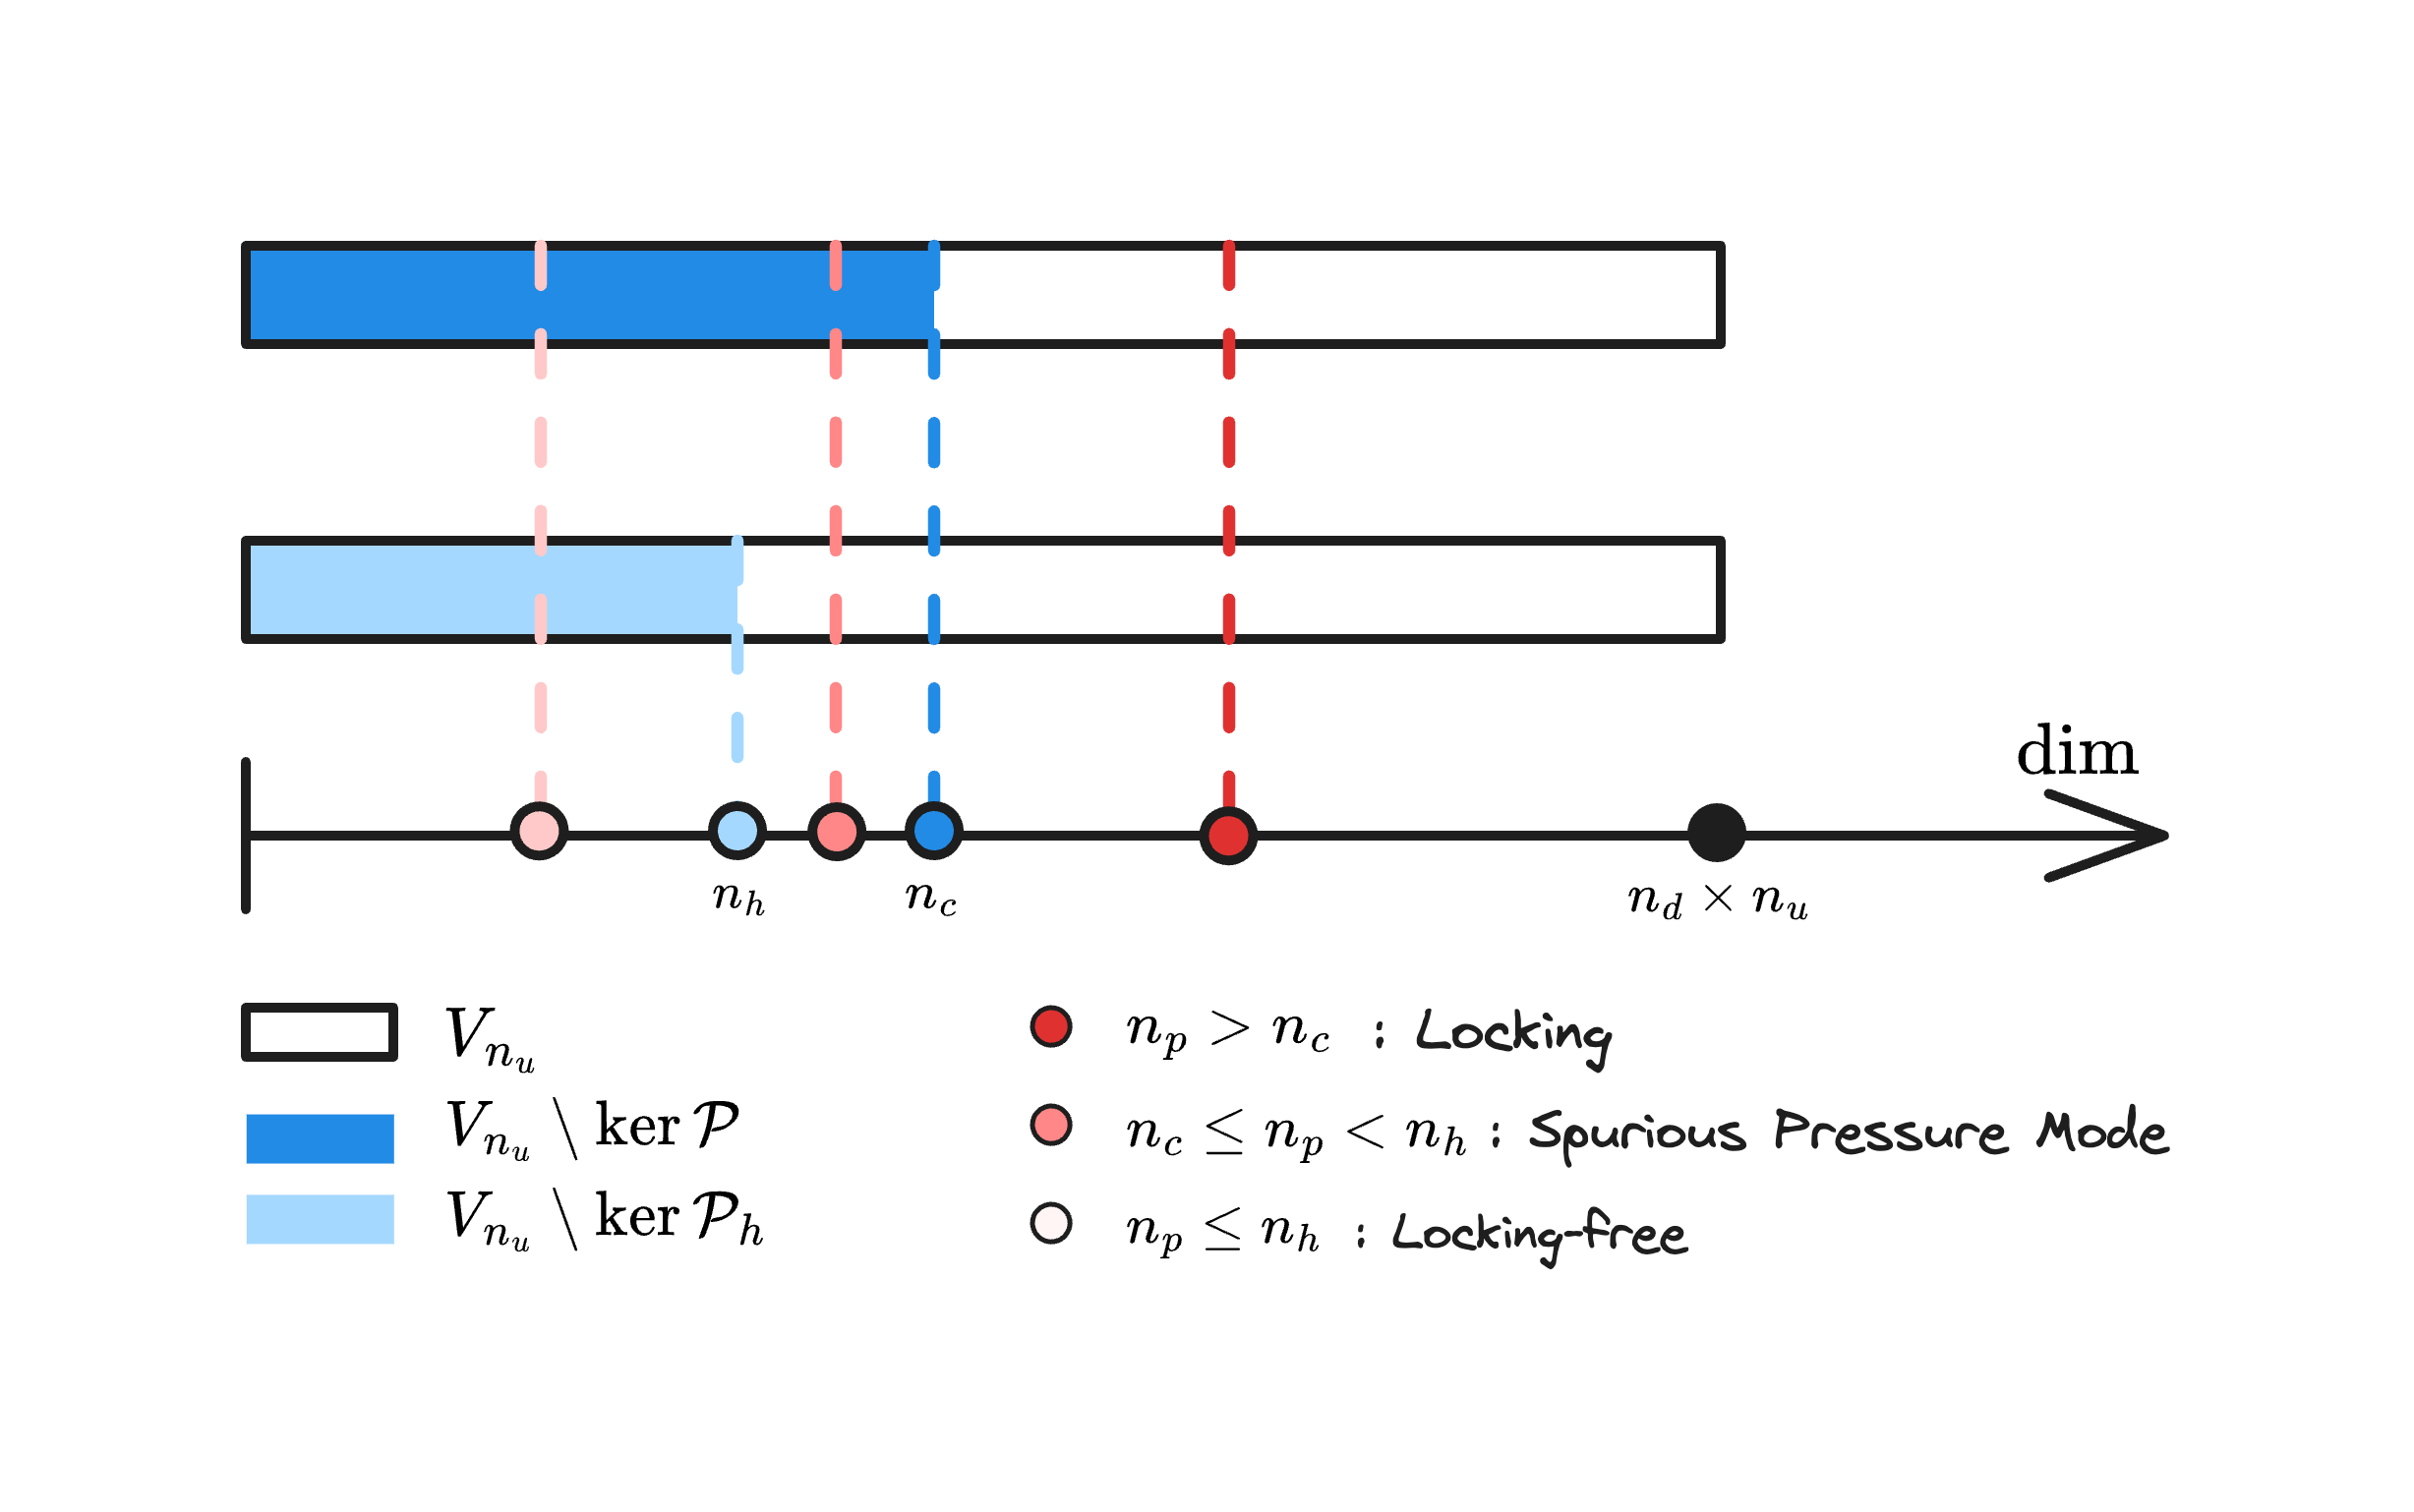
\includegraphics[width=\textwidth]{./png/space.png}
\caption{Illstration for optimal DOFs for pressure}\label{fig:space}
\end{figure}

\begin{itemize}
    \item As $n_p > n_c$, there must exists a subspace in space $V_{n_u}\ker \mathcal P_h \mathcal I_h$ belong to $\ker \mathcal P$, resulting $\beta_2 = 0$. At this circumstance, the LBB condition cannot be satisfied.
    \item As $n_h < n_p \le n_c$, the $\beta_1$ equals to zero, the $\beta$ is bounded appended with $h$. However, considering both the first and second lines of Eq. \eqref{r23}, the reminder $Ch^k$ in first line is not so small and should not be ignored due to $\ker \mathcal P_h \mathcal I_h \subset \ker P$ and $\beta_2 \ne 0$. 
        It will lead to that $\beta$ depend on $h$, $1+\frac{C}{\beta} \approx 1$, thus, from the Eqs. \eqref{ap:estimator1}, \eqref{ap:estimator2}, the solution error will not be polluted by volumetric locking. \cite{bathe2001}

    This case is the typical spurious pressure mode or checkbox mode, a series of stabilization \cite{vadala-roth2020} is proposed to make $\ker \mathcal P \mathcal I_h = \ker \mathcal P$ to eliminate the spurious pressure mode.
\item As $n_p \le n_c$, $(V_{n_u}\setminus \ker \mathcal P_h \mathcal I_h) \subseteq (V_{n_u}\setminus \ker \mathcal P \mathcal I_h) \subseteq (V_{n_u}\setminus \mathcal P)$, now, $\beta$ is a constant independent with $h,s$.
\end{itemize}

    Consequently, the dofs of pressure should remain $n_p\le n_h$ or $n_p\le n_c$ with a stabilizer to release the locking burden. Neitherless, the value of $n_h$ is hard to determine in practice, so the subgrid scale model \cite{hughes1986} is introduced in this work as a stabilization. And $n_c$ can be regarded as the optimal number of optimal volumetric constraint.
\end{pf}

\subsection{Polynomial--wise constraint counting}

For now, $n_c$ can be considered as the optimal pressure's dofs, and the way to determine $n_c$ is shown as follows. For instance, in two dimensional nearly-incompressible elasticity problem, for linear polynomial space with dimension is 3 namely $P_3$, the counterpart displacement space $V_3$ is given by:
\begin{equation}
V_3 = \mathrm{span} \left \{
\begin{pmatrix} 1 \\ 0 \end{pmatrix},
\begin{pmatrix} 0 \\ 1 \end{pmatrix},
\begin{pmatrix} x \\ 0 \end{pmatrix},
\begin{pmatrix} 0 \\ x \end{pmatrix},
\begin{pmatrix} y \\ 0 \end{pmatrix},
\begin{pmatrix} 0 \\ y \end{pmatrix}
\right \}
\end{equation}
or rearranged as follows,
\begin{equation}\label{base1}
V_3 = \mathrm{span} 
\begin{Bmatrix}
\underbrace{
\begin{pmatrix} 1 \\ 0 \end{pmatrix},
\begin{pmatrix} 0 \\ 1 \end{pmatrix},
\begin{pmatrix} y \\ 0 \end{pmatrix},
\begin{pmatrix} 0 \\ x \end{pmatrix},
\begin{pmatrix} x \\ -y \end{pmatrix}
}_{\ker \mathcal P},
\underbrace{
\begin{pmatrix} x \\ y \end{pmatrix}
}_{V_3\setminus \ker \mathcal P}
\end{Bmatrix}
\end{equation}
It can be found from Eq. \eqref{base1}, for $n_u = 3$, $n_c = 1$. Following the path, the displacement space with quadratic polynomial base namely $V_6$ can be stated as:
\begin{equation}\label{base2}
V_6 = \mathrm{span}
\begin{Bmatrix}
\overbrace{
\begin{pmatrix} 1 \\ 0 \end{pmatrix},
\begin{pmatrix} 0 \\ 1 \end{pmatrix},
\begin{pmatrix} y \\ 0 \end{pmatrix},
\begin{pmatrix} 0 \\ x \end{pmatrix},
\begin{pmatrix} x \\ -y \end{pmatrix},
\begin{pmatrix} x^2 \\ -2xy \end{pmatrix},
\begin{pmatrix} y^2 \\ 0 \end{pmatrix},
\begin{pmatrix} 0 \\ x^2 \end{pmatrix},
\begin{pmatrix} -2xy \\ y^2 \end{pmatrix}
}^{\ker \mathcal P}, \\
\underbrace{
\begin{pmatrix} x \\ y \end{pmatrix},
\begin{pmatrix} x^2 \\ 2xy \end{pmatrix},
\begin{pmatrix} 2xy \\ y^2 \end{pmatrix}
}_{V_6\setminus \ker \mathcal P}
\end{Bmatrix}
\end{equation}
In this circumstance, $n_c = 3$. As the order of polynomial space increasing, the every optimal numbers of constraint dofs for each order are listed in Table. \ref{tab:constraint}. 
For the flexibility of usage, the relation between $n_u$ and $n_c$ is summarized as follows:
\begin{equation}
    n_c = \frac{2n_u+1 - \sqrt{1+8n_u}}{2}
\end{equation}
\begin{table}[ht!]
\centering
\caption{Degrees of freedom and volumetric constraint}
\label{tab:constraint}
\begin{tabular}{ccc}
\toprule
    Order of $P_{n_u}$ & $2n_u$ & $n_c$ \\
\midrule
1 & 6 & 1 \\
2 & 12 & 3 \\
3 & 20 & 6 \\
4 & 30 & 10 \\
\vdots & \vdots & \vdots \\
$n$ & $(n+1)(n+2)$ & $\frac{n(n+1)}{2}$ \\
\bottomrule
\end{tabular}
\end{table}

% TODO: discuss about union-jack element arrangement
